\section{Introduction}
Recall the importance of the dot product in space.  Given two vectors $\vecu,\vecv \in \R^3$, we defined the dot product by
\[
\vecu \cdot \vecv = u_1v_1 + u_2v_2 + u_3v_3,
\]
and we also referred to this as an inner product.  The dot product allowed us to project a vector onto its components by, for example,
\[
\vecu \cdot \xhat = u_1.  
\]
This was extremely useful for us.  On top of that, the dot product provided us a means of computing the length of a vector by putting
\[
\|\vecu\|=\sqrt{\vecu\cdot\vecu}.
\]
Underlying much of the theory of space was this structure. 

Later, we introduced the Hermitian inner product on complex vectors.  As it turns out, this inner product is strictly more general than the dot product.  If we had two vectors $\veca,\vecb\in \C^n$ (i.e., vectors with $n$ complex number entries) then we defined the inner product by
\[
\langle \veca,\vecb \rangle = \sum_{j=1}^n a_jb_j^*.
\]
Note that if $\veca$ and $\vecb$ only have real entries, then the complex conjugate $b_j^*=b_j$ and we are left with the typical dot product for $\R^n$.  It suffices to say, that we need only care about this Hermitian inner product. In the same vein, we receive all the wonderful benefits of the dot product.  For example, we can project a vector by taking
\[
\xhat_1 = \begin{pmatrix} 1 \\ 0 \\ 0 \\\vdots \\ 0 \end{pmatrix}
\]
and computing
\[
\langle \veca,\vecx_1\rangle = a_1.
\]
Likewise, the length of a complex vector is given by
\[
\|\veca\|=\sqrt{\langle \veca,\veca\rangle}.
\]
Nothing is lost from this more general approach, and this more general approach extends far beyond finite dimensional complex vectors!

\subsection{Infinite Dimensions}

The dimension of a vector is the number of entries needed to fully describe the vector.  From the examples before, we can say that the vectors $\vecu,\vecv\in \R^3$ are 3-dimensional real vectors and the vectors $\veca,\vecb \in \C^n$ are $n$-dimensional complex vectors.  There is no restriction on the size of $n$, and $n$ can in fact be infinite!

This section of the text is primarily concerned with extending our linear algebra techniques to the infinite dimensional case.  Though this may sound ominous, it simply builds upon what we already know.  In essence, we will combine our knowledge of functions, infinite series, integrals, and linear algebra to complete the theory for infinite dimensions.  Put simply, functions will play the role of vectors while series and integrals will play the role of inner products.  This viewpoint places us viewing mathematics from the top, where we can always reduce the general story to something more specific when need be. Ultimately, this allows one to understand one general structure instead of many individual ones.

\section{Function Spaces}

Rather than leave this section as an abstract approach to more advanced linear algebra, we shall take the viewpoint of working with some specific ideas in mind.  The canonical infinite dimensional vector spaces are formed as spaces of functions.  That is, for example, the set of all solutions to a homogeneous linear ODE of the form
\[
x''(t)+f(t)x'(t)+g(t)x(t)=0.
\]
In the prequel, we proved that any linear combination of solutions to the above equation is also a solution which, along with the fact that $x(t)=0$ is a solution, proves that this set of functions forms a vector space.  

We will not concern ourselves with names for these spaces of functions or their formal definitions.  But, let's list a few more other than the one I mentioned above. Let $\Omega=[0,L]$, then we can consider a few different sets of functions $f\colon \Omega \to \R$ that are vector spaces.
\begin{itemize}
	\item The set of continuous functions.
	\item The set of differentiable functions (whose derivatives are also continuous).
	\item The set of analytic (functions with convergent Taylor series) functions.
	\item The set of functions whose square is integrable. That is, all functions $f$ so that
	\[
		\int_0^L \|f(x)\|^2 dx <\infty.
	\]
	\item The set of solutions to the Schr\"odinger equation for a free particle in a 1-dimensional box.
	\item The set of solutions to the Legendre equation for any nonnegative integer choice of $m$.
\end{itemize}
We will revisit the same spaces again and again as these are prototypes for other problems you will encounter. If you grasp the content for the above examples, seeing it with new examples will not be too challenging.

\section{Inner Products and Norms}

Before we define general inner products, let us recall the definition of a vector space.  In the prequel, we had that a vector space $V$ over some field $\field$ (the numbers we choose as entries) is a set containing vectors that satisfy eight different properties.

\begin{exercise}
	Find the definition in the previous text and review it.
\end{exercise}

\begin{df}{Inner Product}{inner_prod_general}
An \boldgreen{inner product} on a vector space $V$ over a field $\field$ is a bilinear (sometimes sesquilinear) function
\[
\innprod{\cdot}{\cdot} \colon V \times V \to \field,
\]
that satisfies
\begin{enumerate}[i.]
	\item (Nondegenerate) For a $\veca\in V$ we have that $\innprod{\veca}{\veca} =0$ if and only if $\veca=\zerovec$;
	\item (Positive definite) For any nonzero $\veca \in V$ we have that $\innprod{\veca}{\veca} > 0$;
	\item (Symmetric) For any $\veca,\vecb\in V$ we have that $\innprod{\veca}{\vecb} = \innprod{\vecb}{\veca}$. If the vector space is complex, then we have conjugate symmetry $\innprod{\veca}{\vecb}=\innprod{\vecb}{\veca}^*$.
\end{enumerate}
What we are denoting is a function $\innprod{\cdot}{\cdot}$ that has two vectors ($V\times V$) as inputs where see $\cdot$ and outputs some number in the designated field $\field$. When we say bilinear, we mean that the function is linear in each input. For example, we have for vectors $\veca,\vecb,\vecc\in V$ and a scalar $\alpha \in \field$ that
\[
\innprod{\alpha\veca + \vecb}{\vecc} = \alpha \innprod{\veca}{\vecc} + \innprod{\vecb}{\vecc},
\]
which shows the linearity in the first input.  The second input is linear as well.

Similarly, if the field $\field=\C$, then the inner product need be sesquilinear in that we instead have the addition of a complex conjugate in the second position. That is, let $\alpha,\beta\in \C$ and we have
\[
\innprod{\alpha\veca + \vecb}{\beta\vecc} = \alpha \beta^*\innprod{\veca}{\vecc} + \beta^*\innprod{\vecb}{\vecc}.
\]
The first position is simply linear.
\end{df}

\begin{exercise}
	Verify that the dot product for $\R^n$ and the Hermitian inner product for $\C^n$ are indeed inner products.
\end{exercise}

Since we have previously covered two different inner products for the finite dimensional vector spaces $\R^n$ and $\C^n$, we can use our intuition from these spaces with their inner product structure to define other important inner products.  We have in fact come across another example while studying the particle in the 1-dimensional box.  Recall that the problem we solved was the equation
\[
-\frac{\hbar^2}{2m} \frac{d^2 \Psi(x)}{dx^2} = E\Psi(x),
\]
on the region $[0,L]$, where $\Psi(x)$ is the wavefunction.  We also imposed the boundary conditions that $\Psi(0)=\Psi(L)=0$ since the particle cannot be found on the boundary of this domain.  

We found that the solutions to this equation were the normalized states 
\[
\psi_n(x) = \sqrt{\frac{2}{L}} \sin\left(\frac{n\pi x}{L}\right),
\]
with corresponding energies $E_n = \frac{n^2h^2}{8mL^2}$. Then, a wavefunction could be written as a linear combination of these states by
\[
\Psi(x) = \sum_{n=1}^\infty a_n \psi_n(x),
\]
where $a_n \in \C$.  In order for the wavefunction $\Psi(x)$ to be normalized, we required that
\[
\sum_{n=1}^\infty \|a_n\|^2=1.
\]
Now, we can consider a set $V$ of all the possible wavefunctions for the above problem as well as the zero function (which is indeed a solution to the problem, but it is not physically meaningful).

\begin{exercise}
	Show that $V$ is a vector space. 
\end{exercise}

We can add an inner product to the vector space $V$ by defining the inner product on two wavefunctions $\Psi$ and $\Phi$ by
\[
\innprod{\Psi}{\Phi} \coloneqq \int_0^L \Psi(x) \Phi^*(x)dx.
\]
To see that this is an inner product, we need to show that the above function is sesquilinear and satisfies the three conditions for an inner product (nondegeneracy, positive definite, and symmetric).  Sesquilinearity follows from the linearity of the integral in that we have
\begin{align*}
	\innprod{\Psi}{\Phi+\alpha \Theta} &= \int_0^L \Psi(x)(\Phi(x)+\alpha \Theta(x))^*dx \\
	&= \int_0^L \Psi(x) \Phi(x)\Phi^*(x)dx+\alpha^* \int_0^L \Psi(x) \Theta^*(x)dx\\
	&= \innprod{\Psi}{\Phi}+\alpha^* \innprod{\Psi}{\Theta}.
\end{align*}
Showing the linearity in the first argument is analogous but there will not be a complex conjugate.  

Next, we can see that the inner product is nondegenerate by noting that if we take the zero function 0, we have
\[
\innprod{0}{0} = \int_0^L 0 dx = 0,
\]
and if we have that
\[
0=\innprod{\Psi}{\Psi}  = \int_0^L \Psi(x)\Psi^*(x)dx = \int_0^L \|\Psi(x)\|^2dx,
\]
it must be that $\|\Psi(x)\|=0$ since this integral cannot be zero otherwise.  Hence, $\Psi(x)$ is the zero function and we have that the inner product is indeed nondegenerate.

By the above work, if $\Psi(x)$ is not the zero function, then $\|\Psi(x)\|^2>0$ and thus we have
\[
\innprod{\Psi}{\Psi}>0.
\]
Hence, the inner product is positive definite.

Lastly, we can see that the inner product is symmetric by taking the Cartesian representation for $\Psi(x)$ by $\Psi(x)=a(x)+ib(x)$ and for $\Phi(x)=c(x)+id(x)$ and noting
\begin{align*}
	\Psi(x)\Phi^*(x) &= (a(x)+ib(x))(c(x)-id(x))\\
		&= (a(x)c(x)+b(x)d(x))+i(b(x)c(x)-a(x)d(x)),
\end{align*}
and
\begin{align*}
	\Phi(x)\Psi^*(x) &= (c(x)+id(x))(a(x)-ib(x))\\
		&= (a(x)c(x)+b(x)d(x))+i(a(x)d(x)-b(x)c(x),
\end{align*}
which means that we have
\[
\innprod{\Psi}{\Phi}=\innprod{\Phi}{\Psi}^*.
\]
Thus we have shown that this is indeed an inner product.

\subsection{Norms}

We have used the notation $\|\cdot\|$ throughout the prequel and in this text as well. At a first glance, it seems as if it is notationally similar to the absolute value of a real number $|x|$. The reason why we differentiate the notation slightly is that $\|\cdot\|$ means something a bit more general than the absolute value. We call $\|\cdot\|$ a \boldgreen{norm}. For example, the modulus of a complex number $z$ is a norm where we define
\[
\|z\|=\sqrt{zz^*}.
\]
We can also compute the norm of a complex (or real) vector $\vecu$ in $\C^m$ (resp. $\R^m$) by computing 
\[
\|\vecv\| = \sqrt{\innprod{\vecu}{\vecu}}.
\]
In fact, the modulus of a complex number is the special case of $m=1$.  But what is the norm?

The norm of a vector is traditionally referred to as the length of the vector when this vector is something we can picture. For example, the norm of a vector $\vecv \in \R^3$ is given by
\[
\|\vecv = \sqrt{\vecv \cdot \vecv}.
\]
Notice how we are always using an inner product to define a norm! This is a key fact about inner products -- they always induce a norm (or length). 

\begin{remark}
	From here on out we shall use the notation $\innprod{\cdot}{\cdot}$ to refer to the inner product and $\|\cdot\|$ to refer to the induced norm from that inner product.  The choice of inner product should be noted or clear from the choice of vector space.
\end{remark}

	\section{Inner Product Spaces}

Given a vector space $V$ with an inner product, we refer to the vector space as an \boldgreen{inner product space}.  In fact, all the vector spaces we have dealt with are inner product spaces! We tend to prefer working with these spaces as they allow us to nicely compare vectors (like we can with the dot product) and we can also compute lengths and distances.  Needless to say, inner product spaces are immensely important in the physical world.

However, when the vector space is not finite dimensional (such as the space of solutions to the 1-dimensional box with the added zero function), we must be a bit more careful.  Without going into far too much detail, we must add one other attribute to these spaces to make them work as we need.  In this case, we must require that the inner product space is also \boldgreen{complete}.  A space is complete if and only if all Cauchy sequences in the space converge. We call a complete inner product space a \boldgreen{Hilbert space}.

\begin{exercise}
	We defined a Cauchy sequence in the prequel. Find the definition.
\end{exercise}

This extra requirement rules out some oddities and makes the infinite dimensional space much more like the finite dimensional spaces such as $\R^n$ and $\C^n$.  We showed in the prequel that in $\R$ a convergent sequence is also Cauchy. That is, the definitions are analogous. The same happens to be true in $\R^n$ and $\C^n$ (you can picture taking a sequence of vectors instead of a sequence of real numbers).  Thus, in a Hilbert space, Cauchy and convergent are again equal. Let us see why one should believe this.

\begin{ex}{A Cauchy Sequence of Functions}{cauchy_functions}
	Before, we studied power series that define functions.  We would write
	\[
		f(x) = \sum_{n=0}^\infty a_n x^n,
	\]
	where $x$ is in the domain of convergence for the series.  As we worked through what it meant for a series to converge, we found that we could view a series as a sequence of partial sums.  That is, for each value of $x$ we can create a sequence $\{A_n(x)\}_{n=0}^\infty$ by letting
	\[
		A_N(x) = \sum_{n=0}^N a_n x^n.
	\]
	We noted that as we increased $N$, the function $A_N(x)$ became closer and closer to the function $f(x)$.  This was entirely reasonable as if the contrary were true, at some point a large $N$ would provide us a worse approximation to $f(x)$.  

	The completeness assumption for a Hilbert space will give us this ability.  It will allow one to properly approximate quantities such as infinite sums of functions in a way that makes intuitive sense.  
\end{ex}

No more detail is needed on the notion of completeness. We will completely avoid spaces that are not complete as they behave badly.  Take the completeness of any space as given unless it is mentioned otherwise. 

\section{Symmetries}

As previously discussed, symmetry is an important aspect of problem solving that is present in most physical systems.  The prior example is no exception.  We discussed the phase of a complex function and viewed this in an example from quantum mechanics.  There, we found that when a wavefunction is altered by adding a global phase, the probability of making a measurement is not changed.  This is in fact a specific example of something far more general.  But in this case for the particle in the 1-dimensional box, we can see that if alter two wave functions by the same phase and take the inner product
\begin{align*}
\innprod{e^{i\theta} \Psi}{e^{i\theta}\Phi} &= \int_0^L e^{i\theta} \Psi(x) (e^{i\theta}\Phi(x))^*dx \\
	&= \int_0^L e^{i\theta}\Psi(x)e^{-i\theta}\Phi^*(x)dx\\
	&= \int_0^L \Psi(x)\Phi^*(x)dx\\
	&= \innprod{\Psi}{\Phi},
\end{align*}
then the inner product is not changed.  This is an example of a \boldgreen{unitary operator}. A unitary operator preserves the inner product between two vectors. That is, if we have vectors $\Psi$ and $\Phi$ from an Hilbert product space $H$, then $U$ is a unitary operator if $U\colon H \to H$ is onto and
\[
\innprod{U\Psi}{U \Phi} = \innprod{\Psi}{\Phi}.
\]

This is of course not special for just the particle in the 1-dimensional box either. Take the space $\R^2$ with two vectors $\vecu$ and $\vecv$. Then consider a matrix $[A]$ that is in the group $\Orth(2)$ (which means that $[A]$ is a matrix that solely rotates and or reflects vectors).
\begin{exercise}
	Recall the definition of the matrix group $\Orth(2)$.
\end{exercise}
Now, we can actually realize any matrix in $\Orth(2)$ as a reflection matrix, or a product of two reflection matrices. For the sake of example, take a reflection matrix
\[
\REF_\theta = \begin{pmatrix} \cos (2\theta) & \sin(2\theta) \\ \sin(2\theta) & -\cos(2\theta) \end{pmatrix},
\]
which reflects a vector about the line passing through the origin with angle $\theta$ measured from the $x$-axis.  Then letting
\[
\vecu = \begin{pmatrix} u_1 \\ u_2 \end{pmatrix} \qquad \textrm{and} \qquad \vecv = \begin{pmatrix} v_1 \\ v_2 \end{pmatrix},
\]
 we have
\[
\REF_\theta \vecu = \begin{pmatrix} \cos(2\theta)u_1+\sin(2\theta)u_2 \\  \sin(2\theta)u_1-\cos(2\theta)u_2 \end{pmatrix} \qquad \textrm{and} \qquad \REF_\theta \vecv = \begin{pmatrix} \cos(2\theta)v_1+\sin(2\theta)v_2 \\  \sin(2\theta)v_1-\cos(2\theta)v_2 \end{pmatrix}.
\]
\textcolor{red}{Put a picture here}
Then we can compute the inner product of the reflected vectors 
\begin{align*}
\innprod{\REF_\theta \vecu}{\REF_\theta \vecv}&= (\cos(2\theta)u_1+\sin(2\theta)u_2)(\cos(2\theta)v_1+\sin(2\theta)v_2 )\\
&\qquad + (\sin(2\theta)u_1-\cos(2\theta)u_2)(\sin(2\theta)v_1-\cos(2\theta)v_2)\\
&~\vdots\\
&= u_1v_1 + u_2v_2.
\end{align*}
\begin{exercise}
	Show the remaining steps in the above computation.
\end{exercise}
Since this is true for any reflection matrix, it will be true for any product of reflection matrices and hence the group of $\Orth(2)$ matrices are unitary transformations on the inner product space $\R^2$ (where the inner product is the standard dot product).

Every Hilbert space will have a group of unitary symmetries that preserve the inner product. Hence, we tend to have different names for these groups to reflect what the underlying Hilbert product space is. In the particle in a box case, the underlying symmetry is the (slightly inaptly named) unitary group $U(1)$ whereas the case for $\R^2$ it is the orthogonal group $\Orth(2)$.

\section{Bases}

In the case of finite dimensions, we found that we could construct a minimal set of vectors in a space $V$ such that any vector in $V$ can be written as a linear combination of those vectors.  We called such a set a basis.  Take for example, the space $\R^3$, where we had the standard orthonormal basis given by $\xhat$, $\yhat$, and $\zhat$.  We put
\[
\xhat = \begin{pmatrix} 1 \\ 0 \\ 0 \end{pmatrix}, \qquad \yhat = \begin{pmatrix} 0 \\ 1 \\ 0 \end{pmatrix}, \qquad \zhat = \begin{pmatrix} 0 \\ 0 \\ 1 \end{pmatrix},
\]
so that any vector
\[
\vecv = \begin{pmatrix} v_1 \\ v_2 \\ v_3 \end{pmatrix}
\]
could be written as
\[
\vecv = v_1 \xhat + v_2 \yhat + v_3 \zhat.
\]
The latter notation proves to be convenient in the infinite dimensional case.

We have already discovered one way in which we can form a basis for certain infinite dimensional spaces. This came in the form of power series. The major difference is that we have infinite sums to build functions instead of just finite sums to build vectors that live in spaces like $\R^n$ and $\C^n$. 

Let us continue on with the power series example.  For the sake of simplicity, we can consider the space of analytic functions on the region $[0,L]$ (recall that analytic meant the function has a power series).  Then, by definition, every function $f(x)$ in this space can be written as an infinite sum
\[
f(x)=\sum_{n=0}^\infty a_n x^n,
\]
so long as for every $x\in [0,L]$ we have that the above series converges. Thus we have really investigated infinite dimensional spaces and their bases a bit.  In this case, our basis is the set of all powers of $x$. That is to say, we use $\{x^0,x^1,x^2,x^3,\dots\}$ as our basis vectors and the coefficients are the $a_n$.  

In general, the definition of a basis that we have is already correct so long as we understand what it means in general to take a sum. In the previous example with power series, a sum could potentially be infinite.  In some cases (e.g., the Fourier transform) we will see that we may need to take an integral to be our method of summation.  

\subsection{Orthonormal Bases}

Once again, the finite dimensional case led us to discovering the usefulness of an inner product as a method for determining bases that are more useful.  Above, we mentioned the standard orthonormal basis for $\R^3$ which gives us the most natural decomposition of a vector.  Each of the vectors in this basis is of length one and is mutually orthogonal to one another.  Intuitively, this lets you describe a point in space by how much you must walk back or forth, left or right, and up or down to reach your desired location. The orthonormal basis gave us a way to naturally decompose a vector into separate components through the dot product. That is, we could find the $x$, $y$, or $z$-component of a vector and none of these components depend on the others. If you were to take a basis
\[
\vecu = \begin{pmatrix} 1 \\ 1 \\ 0 \end{pmatrix}, \qquad \vecv = \begin{pmatrix} 0 \\ 1 \\ 1 \end{pmatrix}, \qquad \vecw = \begin{pmatrix} 1 \\ 0 \\ 1 \end{pmatrix},
\]
then if you were to break a vector up into these components, you would find that there is some overlap between what each component describes.

\begin{exercise}
	Show the vectors $\vecu$, $\vecv$, and $\vecw$ above form a basis.  Then, to see that there is some overlap, you can find the components of a vector (of your choice) in the directions $\uhat$, $\vhat$, and $\what$. \emph{Hint: to see the overlap, determine the length of the vector you chose, and compare it to the length computed from components un the $\uhat$,$\vhat$, and $\what$.}
\end{exercise}

When a basis is not orthogonal, then to find independent components of a vector, you must somehow subtract off the overlap. This process is a bit tedious, so instead of giving an example, we can just assert the fact that orthogonal bases are indeed helpful. 

\begin{remark}
	Orthogonal bases in finite dimensions also appear when we find eigenvalues and eigenvectors for Hermitian matrices. Specifically, the set of eigenvectors corresponding to different eigenvalues for a Hermitian matrix are always orthogonal!
\end{remark}

One may wish that the Hilbert spaces would have some sense of a natural decomposition into different orthogonal components.  It turns out that in the realm of spaces we care about we can do this, and that some Hilbert spaces have particularly nice bases to work with. In the prequel, we studied series solutions to differential equations as a means of solving a large class of equations. During that time, we solved Legendre's equation and found the solutions were particularly nice.

Recall the equation we wished to solve was
\[
(1-x^2)f''(x)-2xf'(x)+m(m+1)f(x)=0
\]
with our domain $\Omega=[-1,1]$ and $m$ a non-negative integer ($m=0,1,2,\dots$). Ignoring the details, we found that there were solutions for each $m$ (which in some sense are like the eigenvalues for the 1-dimensional box).  The normalized solutions were known as the Legendre polynomials and the first few were
\begin{align*}
	f_0(x)&=\sqrt{\frac{1}{2}} & f_1(x)&=\sqrt{\frac{3}{2}} x\\
	f_2(x)&= \sqrt{\frac{5}{8}} (1-3x^2) & f_3(x)&=\sqrt{\frac{63}{8}}\left(x-\frac{5x^3}{3}\right).
\end{align*}
One may be wondering what we mean by normalized here. The solutions to the Legendre equation live in a Hilbert space whose inner product is given by
\[
\innprod{\Psi}{\Phi} = \int_{-1}^1 \Psi(x)\Phi(x)dx,
\]
in which these functions are normalized. That is, we have  
\[
\|f_i\|= \sqrt{\innprod{f_i}{f_i}} = 1,
\]
for every $i$. Note we do not need a complex conjugate in this inner product since these functions are all real valued. Moreover, it turns out that this set of polynomials is orthonormal since we also have
\[
\innprod{f_i}{f_j} = 0
\]
if $i\neq j$. Finally, the Legendre polynomials form a basis for the solution to the Legendre equation.  Specifically, we can write any other solution as a series of Legendre polynomials by
\[
f(x)= \sum_{n=1}^\infty a_n f_n(x),
\]
so long as the series converges for all values of $x$ in the domain $\Omega$.  

In the realm of quantum mechanics, the orthonormal basis of eigenfunctions are extremely important. Previously, we even donated these functions with the term \boldgreen{states}.  Though we never defined this term in the prequel, we now have a rough working definition.  When observing a quantum system, it is only possible to observe a particle in an eigenstate of the operator that is mathematical representation for the observation you are wishing to make.  We will define operators, eigenfunctions, and observables later.

Another example of a basis arises from the solutions to the free particle in the 1-dimensional box.  If we let the Hilbert space be any solution to the boundary value problem along with the zero solution which we ruled out as not being physically meaningful (it is a solution, just not physically), then we found the orthonormal basis was given by all the states
\[
\psi_n(x) = \sqrt{\frac{2}{L}}\sin\left(\frac{n\pi x}{L}\right).
\]
Hence, any solution to that problem can be written as
\[
\Psi(x) = \sum_{n=1}^\infty a_n \psi_n(x),
\]
so long as this sum converges for $x$ values in the domain $[0,L]$.

\subsection{Series and Integrals as Linear Combinations}

The two main points of a basis is really to give us a way to extract interesting components of a vector and to be able to uniquely write any vector as a linear combination of the fewest possible elements of a vector space.  As discussed above, we can make our lives easiest by choosing nicer bases such as bases that are orthonormal.  Let us assume that we will do this.

For certain Hilbert spaces $\hilbert$, we can write any vector in the space as a sum or series.  First, take for example, $\R^n$. Let us choose the orthonormal basis
\[
\xhat_1 = \begin{pmatrix} 1 \\ 0 \\ 0 \\ \vdots \\ 0 \end{pmatrix}, \qquad \xhat_2 = \begin{pmatrix} 0 \\ 1 \\ 0 \\ \vdots \\ 0 \end{pmatrix},\quad \dots, \quad \xhat_n = \begin{pmatrix} 0 \\ 0 \\ 0 \\ \vdots 0 \end{pmatrix}.
\]
Then we can write any vector in the space $\R^n$ as a finite sum of the basis elements above by
\[
\vecv = \sum_{i=1}^n v_i \xhat_i = v_1 \xhat_1 + v_2 \xhat_2 + \cdots + v_n \xhat_n = \begin{pmatrix} v_1 \\ v_2 \\ v_3 \\ \vdots \\ v_n \end{pmatrix}.
\]
As always, the $\xhat_i$ form the basis for $\R^n$ and the $v_i$ are the coefficients for the vector $\vecv$.

When $\hilbert$ is infinite dimensional, we can no longer easily manipulate vectors as column vectors (it just doesn't always make sense)! So, we our hand is forced and we must write our vectors as some form of an infinite sum.  Of course, this is just an infinite version of a linear combination! For now, let us assume $H$ is sufficiently nice\footnote{Sufficiently nice here means \boldgreen{separable}. Do not worry about this definition!} so that we can write any vector $\Psi\in \hilbert$ by
\[
\Psi = \sum_{i=1}^\infty a_n \psi_n
\]
where the collection of all $\psi_n$ is a basis for $H$ and the $a_n$ are the coefficients for $\Psi$.  Not much has changed here, but the sum has now become infinite so we must handle convergence with care! One may also find that the infinite sum may not converge to the intended function at \emph{every} point in the domain (but this is a non-issue). We will see this when we cover the Fourier series.

Finally, for the Hilbert spaces that are not quite as nice, we may in fact need to use integration as our form of linear combination.  We will see this in the case of the Fourier transform where we must put
\[
f(x)=\int_{-\infty}^\infty \hat{f}(\omega) \chi_x(\omega)d\omega.
\]
Here, the basis elements are the $\chi_x(\omega)$ which for the Fourier transform have the form
\[
\chi_x(\omega) = e^{i\omega x}.
\]
The coefficients are then given by the function $\hat{f}(\omega)$ where, for example, $\omega \in \R$. This is analogous the the above cases, its just that the list of coefficients is not finite, or indexed by integers, but rather it is indexed by the whole (larger) set of real numbers $\R$.  

\begin{remark}
	There is much going on here. Much if it is coming down to the sizes of infinities and underlying spaces we are working with.  The point is to see that we are solely generalizing the notion of writing a vector in a basis. Some spaces just have a very large amount of basis elements!	
\end{remark}

\subsection{Projection}

When we are handed a vector $\vecv\in \R^3$ we can recover the components of $\vecv$ by projecting onto our orthonormal basis.  As I've said before, we do this by
\[
\vecv \cdot \xhat = v_1.
\]
Nothing changes when we work with an infinite orthonormal basis.  Say we have the basis $\psi_n$ for some Hilbert space,  then for a vector $\Psi$, we can recover the component $a_n$ by
\[
\innprod{\Psi}{\psi_n}=a_n.
\]
This is a surprisingly helpful fact.

Sometimes, we want to see what the fundamental components of a function are in order to approximate a function.  We did this with power series, but this is not always the best choice.  We also have developed machines that work via extracting, for example, frequency components of functions (see Fourier transform spectroscopy).  If one is able to find that a complicated function is well approximated by the sum of a few far less complicated functions, this will simplify the analysis we do when we work with the function. Let us work with an example.

\begin{ex}{Triangle Wave}{triangle_wave}
	Let's consider the function $f\colon [0,L]\to \R$ given by
	\[
		f(x)=\begin{cases} x & 0\leq x\leq L/2\\ L-x & L/2<x\leq L\end{cases}
	\]
	We wish to find a suitable orthonormal basis of functions with domain $[0,L]$.  In this case, let us define the inner product by
	\[
	\innprod{g}{h} = \frac{1}{L}\int_0^L g(x)h(x)dx,
	\]
	which is a scaled version of the Hermitian inner product (with omitted conjugate since the functions are real).  We will revisit this inner product when we arrive at Fourier series.  

	Now, since this is a scaled version of the Hermitian inner product and since $f(x)$ satisfies the zero boundary conditions requirement, we can conjecture that a suitable orthogonal basis is given by
	\[
		\sin\left( \frac{n\pi x}{L}\right)
	\]
	where $n=1,2,3,\dots$. We know that these elements are orthogonal in that
	\[
		\innprod{\sin\left( \frac{n\pi x}{L}\right)}{\sin\left( \frac{m\pi x}{L}\right)}=0
	\]
	when $n\neq m$.  However, we must normalize these vectors as well since our inner product is not the same.  We take
	\begin{align*}
		1&=\innprod{c\sin\left( \frac{n\pi x}{L}\right)}{c\sin\left( \frac{n\pi x}{L}\right)}\\
		&= \frac{1}{L} \int_0^L c^2 \sin^2\left(\frac{n\pi x}{L}\right)dx\\
		&= \frac{c^2}{2}.
	\end{align*}
	We can then solve for the normalization constant $c$ to find that we get $c=\sqrt{2}$.  Hence we have that our orthonormal basis for this inner product is
	\[
		\psi_n(x)= \sqrt{2} \sin \left(\frac{n \pi x}{L}\right),
	\]
	for $n=1,2,3,\dots$. Now, we have our $f(x)$, and we want to extract the components of $f(x)$.  To do this, we use the inner product and project by
	\begin{align*}
		a_n&=\innprod{f}{\psi_n}\\
			&= \frac{1}{L} \int_0^L f(x) \sqrt{2} \sin\left(\frac{n\pi x}{L}\right)dx\\
			&= \sqrt{2}\left(\frac{L\sin\left(\frac{\pi n}{2}\right)-\frac{1}{2}\pi Ln\cos\left(\frac{\pi n}{2}\right)}{\pi^{2}n^{2}}
+\frac{L\left(2\sin\left(\frac{\pi n}{2}\right)+\pi n\cos\left(\frac{\pi n}{2}\right)\right)}{2\pi^{2}n^{2}}\right).
	\end{align*}
	You should verify the integral above.

	What this means is that we can now put
	\[
		f(x) = \sum_{n=1}^\infty \sqrt{2}\left(\frac{L\sin\left(\frac{\pi n}{2}\right)-\frac{1}{2}\pi Ln\cos\left(\frac{\pi n}{2}\right)}{\pi^{2}n^{2}}
+\frac{L\left(2\sin\left(\frac{\pi n}{2}\right)+\pi n\cos\left(\frac{\pi n}{2}\right)\right)}{2\pi^{2}n^{2}}\right) \sqrt{2}\sin\left(\frac{n\pi x}{L}\right).
	\]
	The question now is whether this is believable at all. Because, let's face it, this seems pretty odd. So, let's examine what these functions look like.

	There is no nice way of evaluating the above infinite sum, but we can take finite sum approximations from this. For example, we can choose some positive integer $N$ and take
	\[
		f(x)\approx \sum_{n=1}^N a_n \psi_n(x).
	\]
	Let us plot various degrees of approximations with the original function $f(x)$.

	\begin{figure}[H]
	\centering
		\begin{subfigure}[h]{0.49\textwidth}
			\centering
			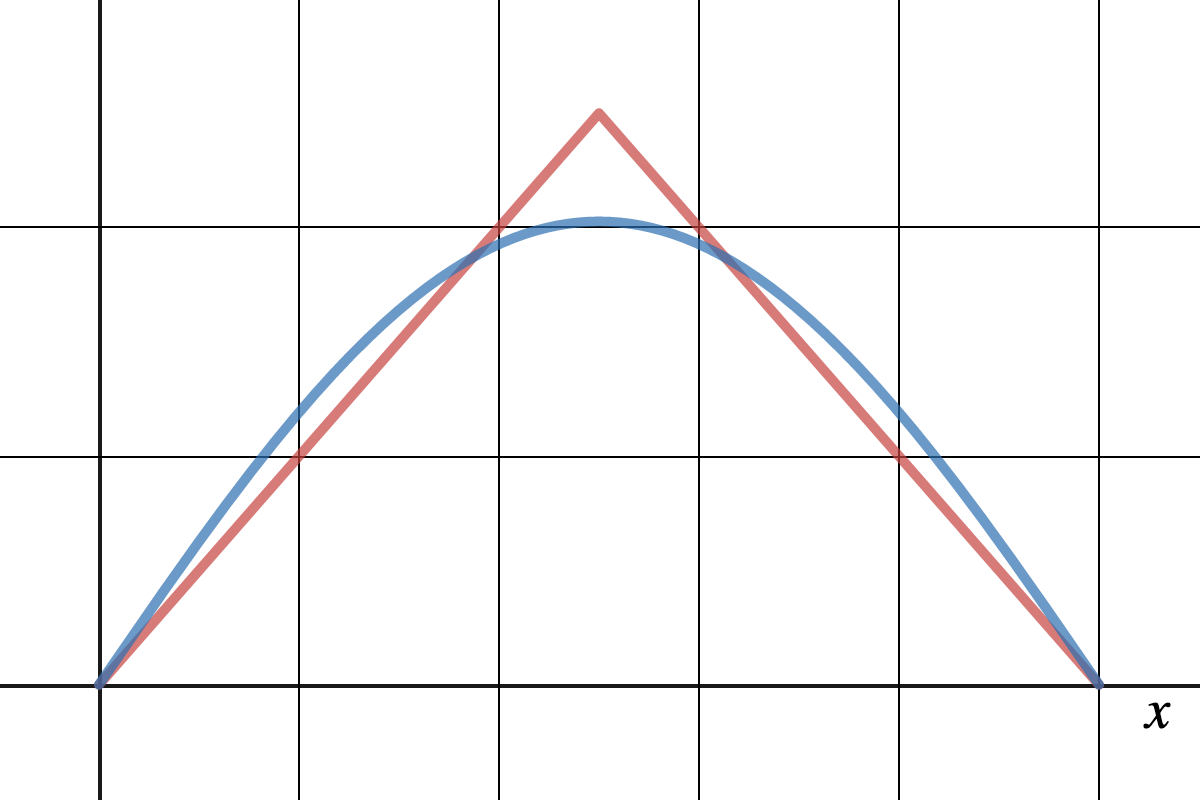
\includegraphics[width=.8\textwidth]{Figures_Part_5/triangle_n=1.png}
			\caption{Approximation of $f(x)$ with $n=1$ basis elements..}
		\end{subfigure}
		~
		\begin{subfigure}[h]{0.49\textwidth}
			\centering
			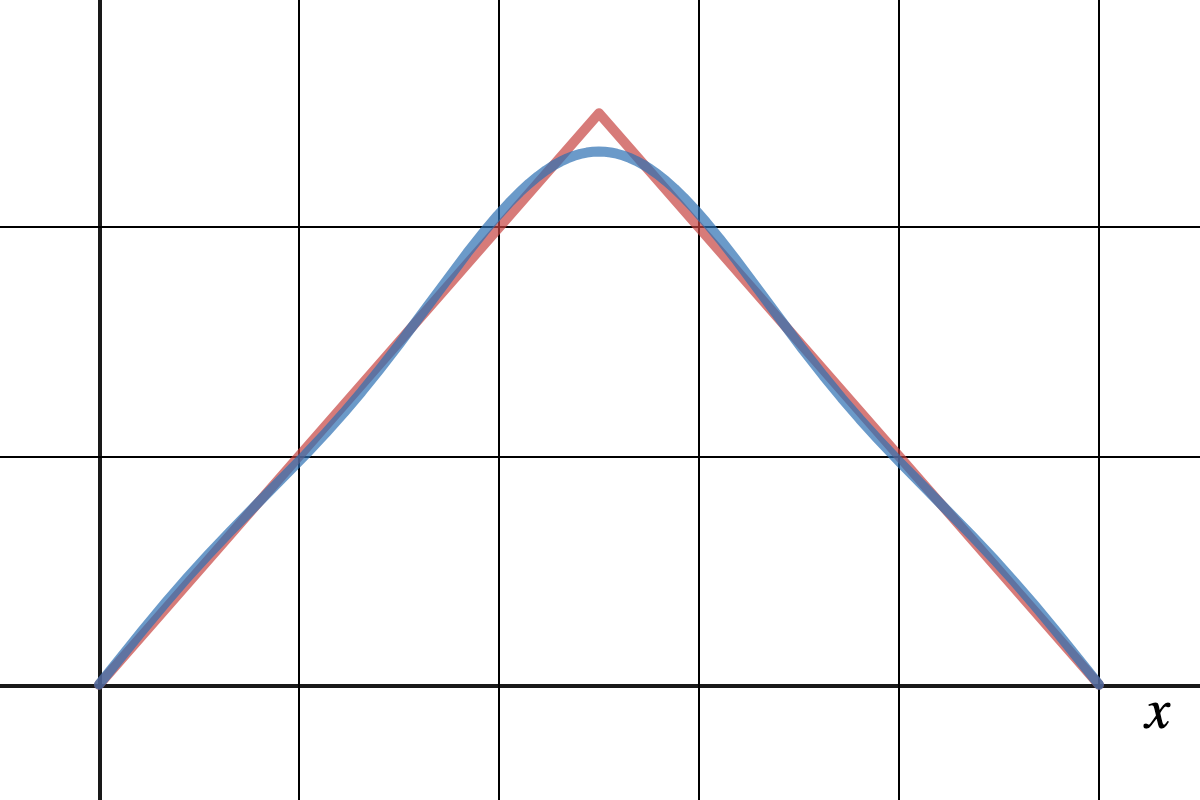
\includegraphics[width=.8\textwidth]{Figures_Part_5/triangle_n=5.png}
			\caption{Approximation of $f(x)$ with $n=5$ basis elements.}
		\end{subfigure}
		\\
		\begin{subfigure}[h]{0.49\textwidth}
			\centering
			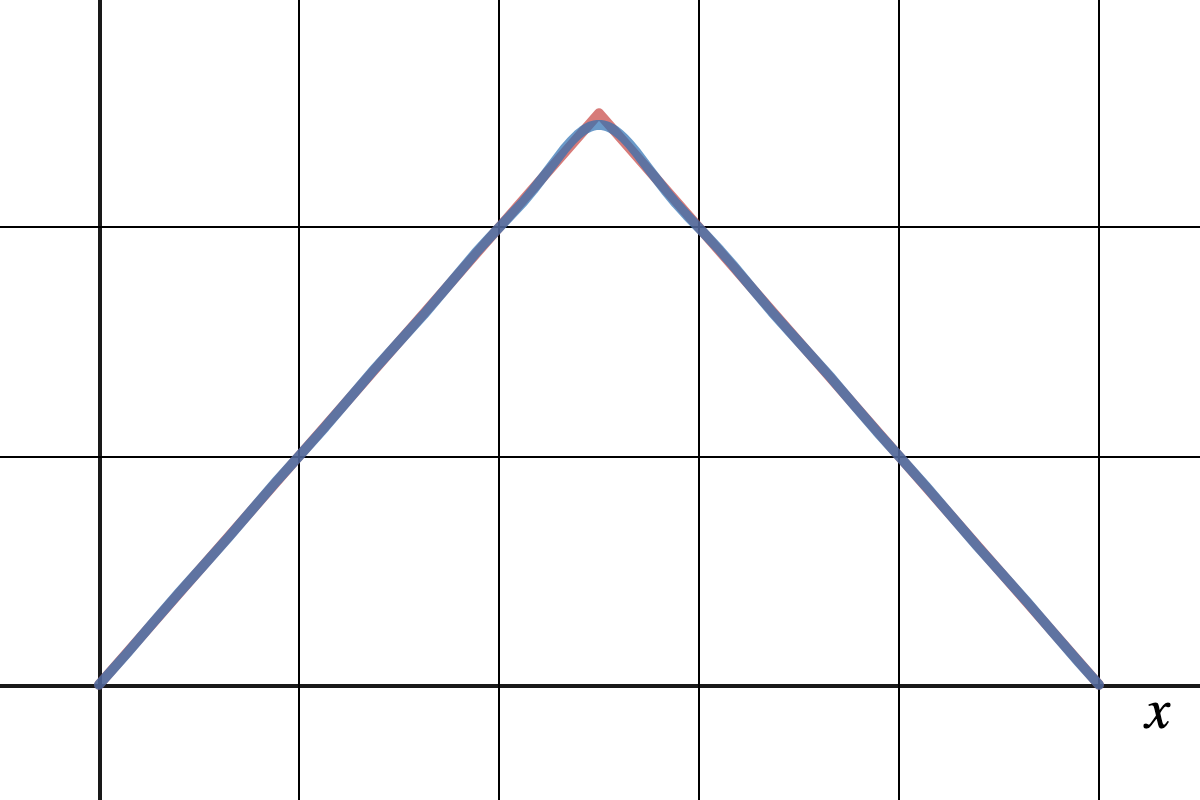
\includegraphics[width=.8\textwidth]{Figures_Part_5/triangle_n=20.png}
			\caption{Approximation of $f(x)$ with $n=20$ basis elements.}
		\end{subfigure}
		~
		\begin{subfigure}[h]{0.49\textwidth}
			\centering
			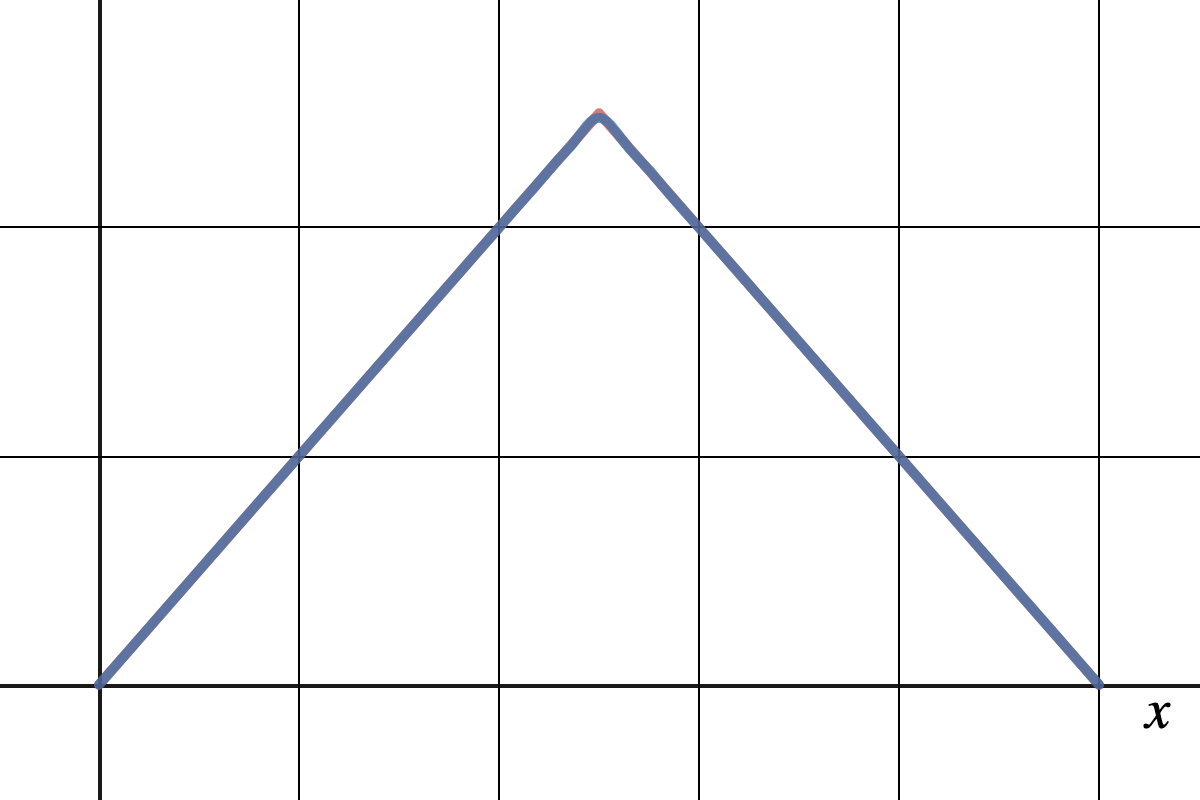
\includegraphics[width=.8\textwidth]{Figures_Part_5/triangle_n=50.png}
			\caption{Phase difference $\delta=\pi$.}
		\end{subfigure}
	\caption{Approximation of $f(x)$ with $n=50$ basis elements.}
	\end{figure}

	The above example is of dire importance in the realm of experimentation.  If we were not able to approximate functions using a methodology like this, all computation would be far more difficult and possible infeasible. One can see from the above example that an approximation with 20 or more terms is fantastic.  What we have done here is also important for modelling differential equations. For example, in some equations, one can take the first 20 basis functions and see how the coefficients $a_n$ change over time as opposed to explicitly solving the differential equation. This is the essence of finite element approaches.
\end{ex}


	
	
